\chapter{\trys{} Screenshots}
\label{appendix:screenshots}

Below are the following desktop screenshots:
\begin{itemize}
    \item The landing page for \trys{}: Figure~\ref{screenshot:landing-desktop}. Exists to direct users to either the documentation/tutorial or open the learning environment.
    \item The default editor: Figure~\ref{screenshot:editor-desktop}. This is the environment that loads by default, the loaded code, if run, draws a version of the main logo.
    \item A game of snake in progress: Figure~\ref{screenshot:snake-desktop}.
    \item The documentation site (Irish section): Figure~\ref{screenshot:docs-ga-desktop}.
\end{itemize}
Then follows the following mobile screenshots:
\begin{itemize}
    \item The landing page for \trys{}: Figure~\ref{screenshot:landing-mobile}.
    \item The Sierpinski triangle demo running on mobile: Figure~\ref{screenshot:sierpinski-mobile}.
    \item The Setanta documentation (English): Figure~\ref{screenshot:docs-en-mobile}.
\end{itemize}

\begin{center}
    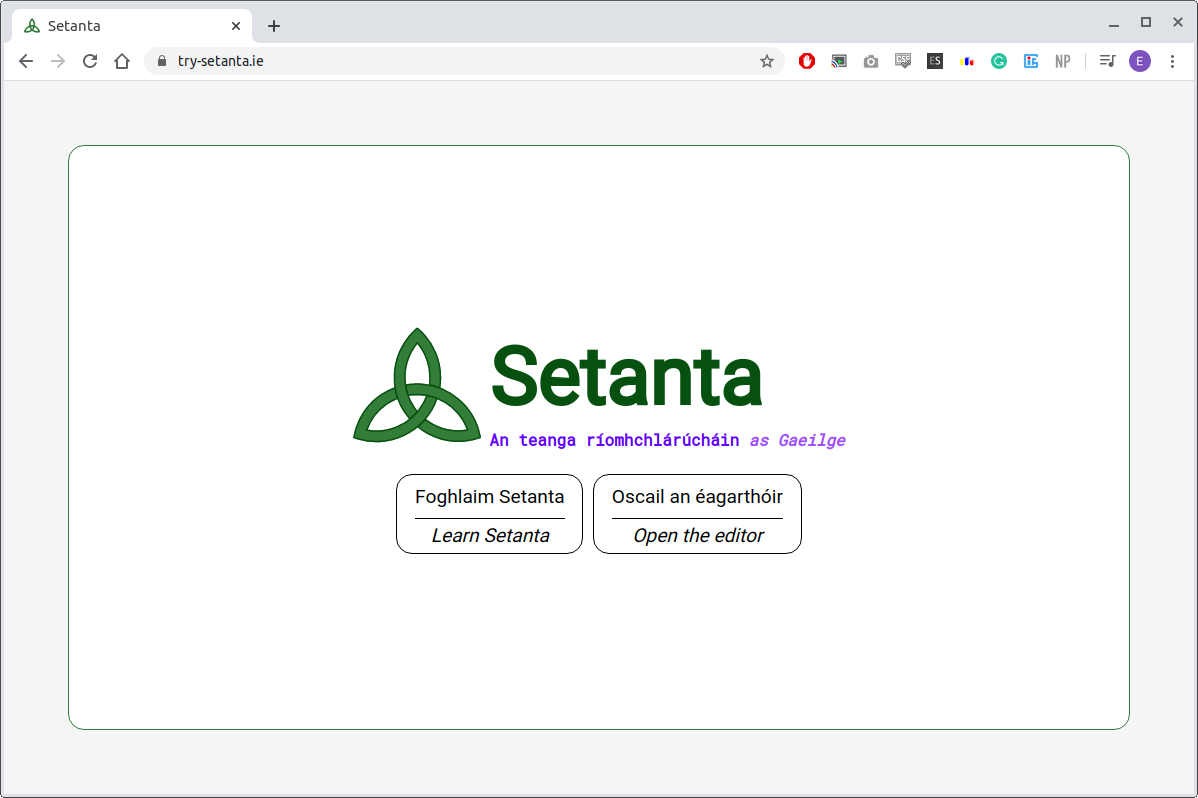
\includegraphics[scale=0.38]{app4assets/landing-desktop}
    \captionof{figure}{Test}
    \label{screenshot:landing-desktop}
\end{center}

\begin{center}
    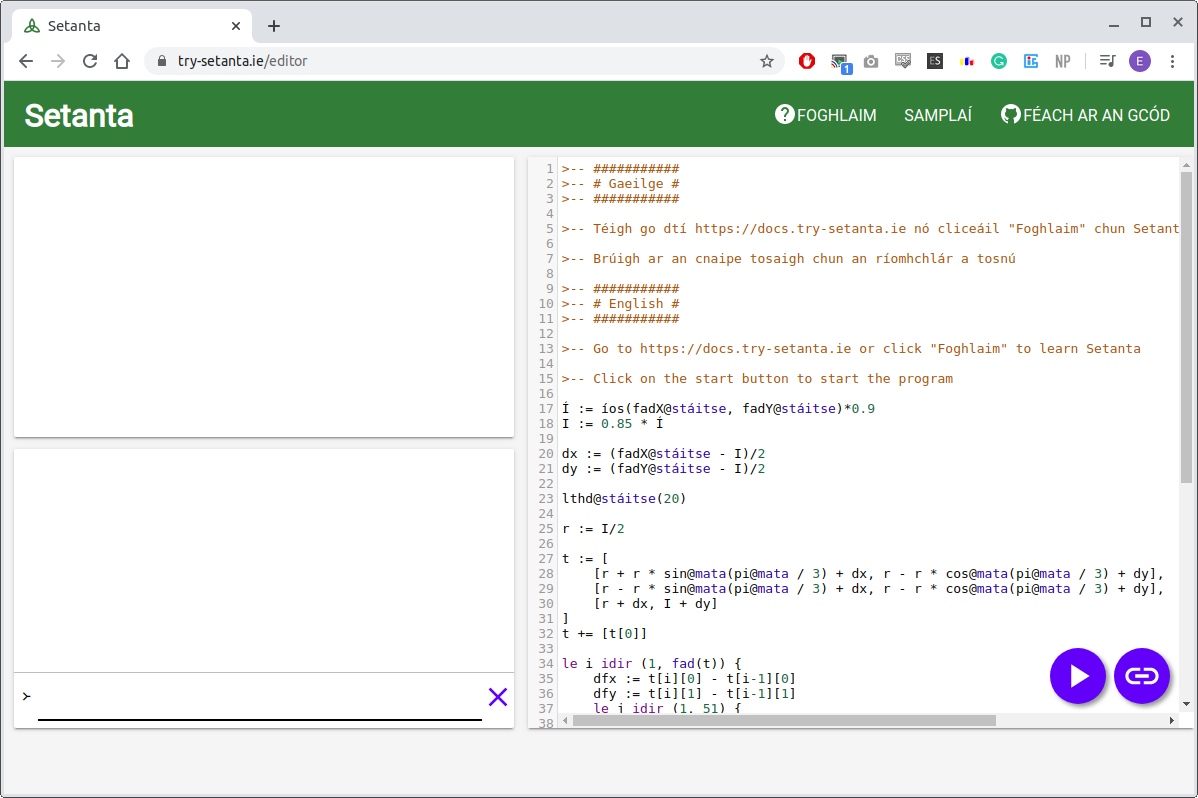
\includegraphics[scale=0.38]{app4assets/editor-desktop}
    \captionof{figure}{Default editor page}
    \label{screenshot:editor-desktop}
\end{center}

\begin{center}
    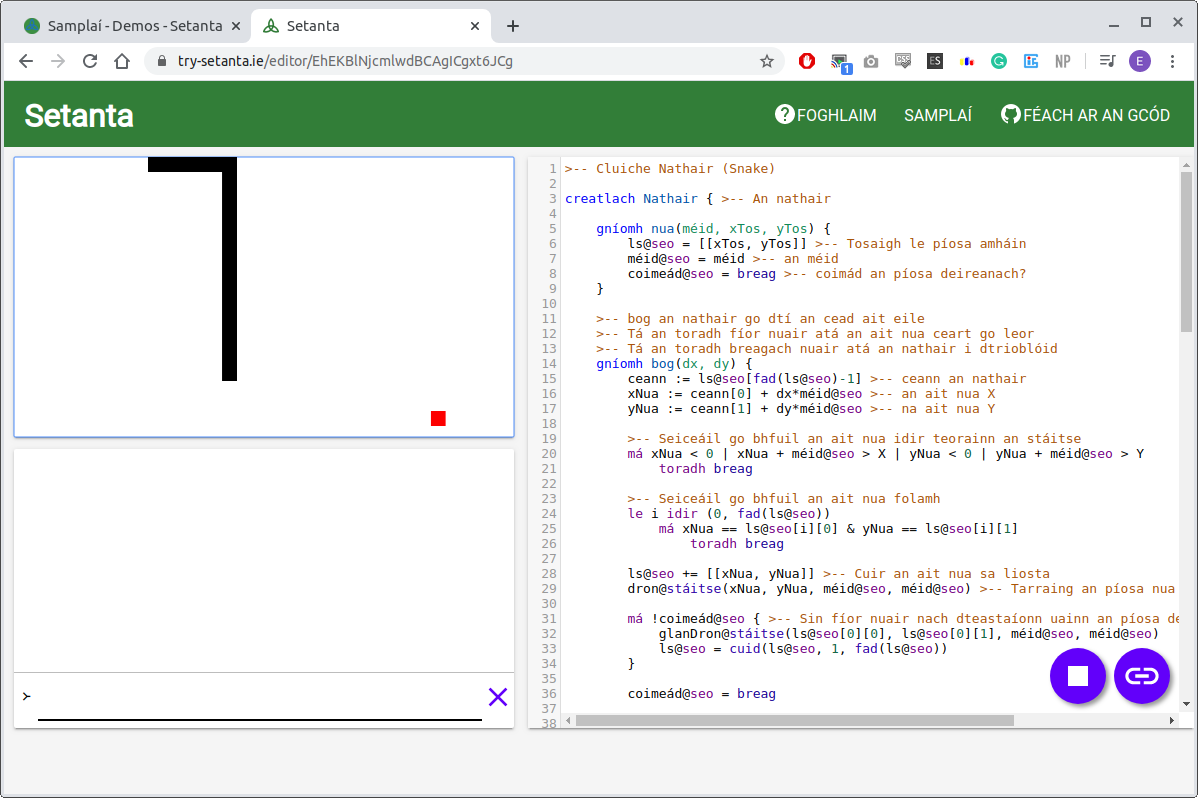
\includegraphics[scale=0.38]{app4assets/snake-desktop}
    \captionof{figure}{Snake game in progress}
    \label{screenshot:snake-desktop}
\end{center}

\begin{center}
    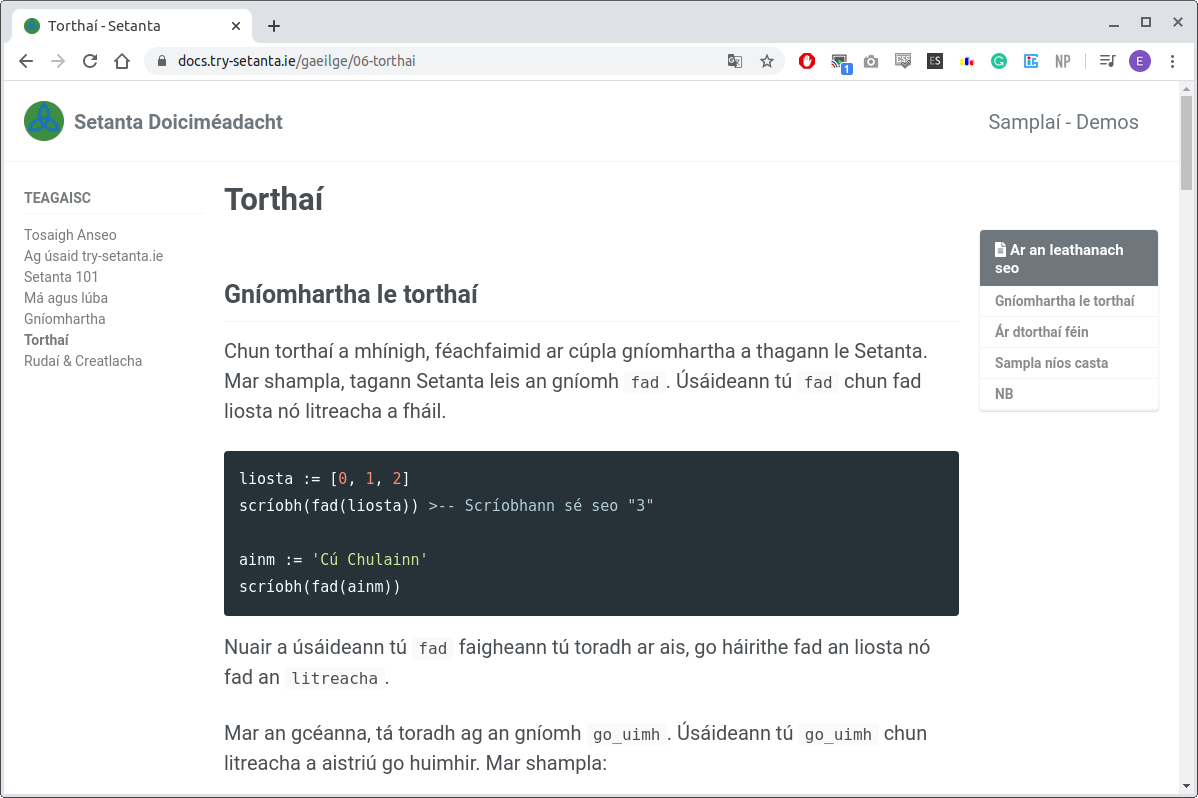
\includegraphics[scale=0.38]{app4assets/docs-ga-desktop}
    \captionof{figure}{Documentation site (Irish section)}
    \label{screenshot:docs-ga-desktop}
\end{center}%
%
\fbox{
\begin{minipage}[t]{0.32\textwidth}
    \begin{center}
        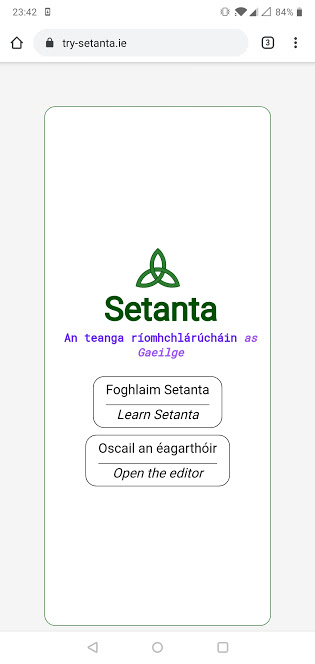
\includegraphics[scale=0.4]{app4assets/landing-mobile}
        \captionof{figure}{Landing page on mobile}
        \label{screenshot:landing-mobile}
    \end{center}
\end{minipage}
}
\hspace{0.5mm}
\fbox{
\begin{minipage}[t]{0.32\textwidth}
    \begin{center}
        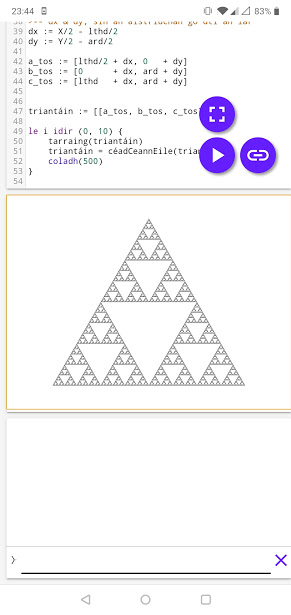
\includegraphics[scale=0.43]{app4assets/sierpinski-mobile}
        \captionof{figure}{Sierpinski triangle demo running on mobile}
        \label{screenshot:sierpinski-mobile}
    \end{center}
\end{minipage}
}
\hspace{0.5mm}
\fbox{
\begin{minipage}[t]{0.32\textwidth}
    \begin{center}
        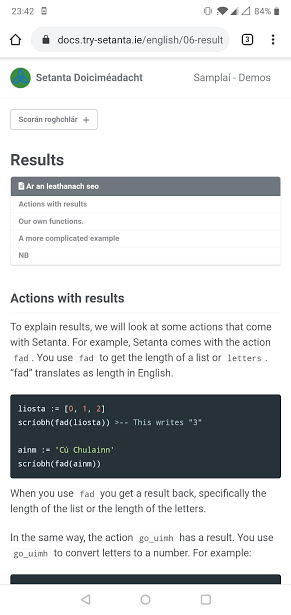
\includegraphics[scale=0.43]{app4assets/docs-en-mobile}
        \captionof{figure}{Setanta documentation mobile (English)}
        \label{screenshot:docs-en-mobile}
    \end{center}
\end{minipage}
}
